\documentclass{article}
\usepackage[utf8]{inputenc}
\usepackage{polski}
\usepackage[fleqn]{amsmath}
\usepackage{newlfont}
\usepackage{hyperref}
\usepackage[dvips]{graphicx}
\title{Pierwsze przeloty szybowcowe}
\author{Osowski~Marcin\\Aeroklub~Warmińsko-Mazurski}
\hypersetup{
    pdftitle={Pierwsze przeloty szybowcowe},    % title
    pdfauthor={Osowski Marcin},     % author
    colorlinks=true,          % false: boxed links; true: colored links
    linkcolor=black,          % color of internal links
    citecolor=black,          % color of links to bibliography
    filecolor=black,          % color of file links
    urlcolor=black            % color of external links
}

\newenvironment{packed_enum}{
\begin{enumerate}
  \setlength{\itemsep}{1pt}
  \setlength{\parskip}{0pt}
  \setlength{\parsep}{0pt}
}{\end{enumerate}}


\begin{document}

\maketitle
\newpage

\begin{abstract}
W tym opracowaniu zebrałem garść informacji dla pilotów szybowcowych
pragnących opuścić stożek dolotowy i rozpocząć
przygodę przelotową. Informacje tu zawarte bazują na moim
własnym doświadczeniu i cudzych opiniach, których autorstwo jest na ogół
trudne do ustalenia. Treść została podzielona na trzy części:
przygotowanie do przelotu, taktyka przelotowa, 
lądowanie w terenie przygodnym i postępowanie po lądowaniu.
\end{abstract}
\newpage

\begin{center}\begin{huge}
Zrzeczenie się odpowiedzialności
\end{huge}\end{center}
Informacje zawarte w niniejszym opracowaniu oparte są o obserwacje
autora i inne tego typu opracowania; mają znaczenie wyłącznie informacyjne
i edukacyjne. Pomimo dołożenia wielu starań nie mogą być stosowane
jako porady i nie mogą być podstawą roszczeń wobec autora,
Aeroklubu Warmińsko-Mazurskiego ani kogokolwiek rozprzestrzeniającego
ten dokument.
\newpage


\tableofcontents
\newpage


\section{Wstęp, czyli grupa odbiorców tego opracowania}
Opracowanie to jest skierowane do pilotów i uczniów-pilotów o niewielkim
doświadczeniu. Wymaga jednak znajomości podstaw latania szybowcowego, w tym
pewnego doświadczenia w lataniu termicznym.
\newpage


\section{Przygotowania do przelotu}
Zacznijmy od wypunktowania tego co należy przygotować wcześniej.

\subsection{Lista rzeczy do zrobienia wcześniej}
Potrzebujesz:
\begin{enumerate}
\item aeroklubowej zgody na przelot szybowcem
\item pomocy nawigacyjnych
\item przygotowanego wózka transportowego
\item przygotowanego telefonu komórkowego
\item (do lotów warunkowych) rejestratora
\end{enumerate}

\subsubsection{Aeroklubowa zgoda na wykonanie przelotu}
Tradycyjnie w Aeroklubie Warmińsko-Mazurskim przed jakimkolwiek przelotem
wymaga się od uczniów-pilotów zdobycia przewyższenia 1000 m oraz wykonania
co najmniej pięcio-godzinnego lotu szybowcem. Dodatkowo, każdy pilot musi
przygotować się do lądowania poza lotniskiem -- oznacza to wykonanie co
najmniej dziesięciu lądowań na typie szybowca na którym planowany jest
przelot.

Pamiętaj, że warunki pogodowe i stan upraw na polach mogą cię zaskoczyć,
dlatego zawsze konsultuj swoje plany z Szefem Wyszkolenia oraz innymi
doświadczonymi pilotami.

\subsubsection{Pomoce nawigacyjne}
Musisz mieć mapę. Mapa powinna mieć skalę
w granicach od 1:750~000 do 1:200~000. Mniejsze skale utrudniają
nawigację, natomiast na mapach o większej skali będziesz miał/miała
problem z przekładaniem stron podczas lotu.

Jak należy przygotować mapę? Na mapie trzeba zaznaczyć okręgi
wokół lotniska, o promieniach
na przykład co 5 km. Okręgi te powinny być opisane minimalnymi
wysokościami gwarantującymi dolot. Jak określić minimalną wysokość?
Spróbujmy oszacować doskonałość osiąganą przez szybowiec w rzeczywistych
warunkach. Rozpatrzmy dwa warianty, oba dla szybowca Junior:

\begin{enumerate}
\item Załóżmy, że warunki są bezwietrzne (albo szybowiec jest po
    nawietrznej stronie lotniska), a średnie duszenie netto
    (czyli ponad opadanie własne szybowca) ma wartość
    $-0,5 \frac{m}{s}$. Czyli warunki bardzo spokojne. Krążek przelotowy
    wskazuje jako optymalną prędkość $100 \frac{km}{h}$. Daje
    to całkowite opadanie szybowca $-1,5 \frac{m}{s}$. Doskonałość:
    \begin{align*}
        \frac{100 \frac{km}{h}}{1,5 \frac{m}{s}} = 18,5
    \end{align*}

\item Weźmy teraz zdecydowanie bardziej niekorzystne warunki. Czołowy
    wiatr $20 \frac{km}{h}$, duszenie netto $-1,0 \frac{m}{s}$.
    Według krążka optymalna prędkość to $130 \frac{km}{h}$.
    Odejmujemy od tego prędkość wiartu, wychodzi $110 \frac{km}{h}$.
    Całkowite opadanie szybowca: $2,5 \frac{m}{s}$. Doskonałość:
    \begin{align*}
        \frac{110 \frac{km}{h}}{2,5 \frac{m}{s}} = 12,22
    \end{align*}
\end{enumerate}

\noindent
Widać stąd, jak trudno jest osiągnąć książkową doskonałość juniora: $35$.

Aby określić bezpieczną wysokość dolotu należy założyć co nieco na temat warunków.
Przy założeniu braku wiatru (albo pozostawania po nawietrznej stronie lotniska)
dobrym ograniczeniem dla doskonałości jest $15$. Ponadto, potrzeba 300 metrów
aby wykonać krąg do lądowania. Zatem na okręgu o promieniu $5 \textrm{ km}$ potrzebujesz:
\begin{equation*}
300\textrm{ m}+\frac{5\textrm{ km}}{15} = 630 \textrm{ m}
\end{equation*}
\noindent
Podobne obliczenia trzeba wykonać dla okręgów o pozostałych promieniach.
Należy mieć na uwadze, że powyższe obliczenia nie obejmują sytuacji dolotu
pod wiatr! Przy silnym wietrze zasięg szybowca może drastycznie zmaleć,
nawet względem doskonałości $15$.

Przykład przygotowanej mapy znajdziesz w punkcie opisującym przygotowanie
trasy.

Popularną pomocą nawigacyjną jest PDA (nazwa zwyczajowa: ,,lusterko'') 
wykonujący program przystosowany
do potrzeb szybowników. Na rynku jest dostępnych co najmniej 5
rozwiązań:
\begin{enumerate}
\item GPS\_LOG -- darmowy
\item LK8000 -- damowy
\item SeeYou Mobile
\item WinPilot
\item XCSoar -- darmowy
\end{enumerate}
Moje doświadczenia ograniczają się do punktu 2. i punktu 4., ale
opinie o każdym z wyżej wymienionych programów są pozytywne.

\subsubsection{Przygotowany wózek transportowy}
Należy liczyć się z lądowaniem poza lotniskiem. 
Wózek transportowy musi być sprawny i posiadać wszystkie wymagane
dokumenty (świadectwo rejestracji, ważne ubezpieczenie OC). Dobrze jest
umówić się z kimś co do ewentualnego transportu szybowca z pola -- po
lądowaniu zazwyczaj mamy mniejsze możliwości uzgadniania takich kwestii.

Przydatnym zwyczajem jest zabieranie ze sobą do szybowca kliku metrów
linki transportowej. Zdarza się, że lądujemy na polu w pobliżu którego
rolnicy wykonują jakieś prace -- można wtedy poprosić ich o ściągnięcie
szybowca na skraj pola.

\subsubsection{Przygotowany telefon komórkowy}
Oczywiście na wypadek lądowania w polu. Zapisz sobie w książce adresowej
numery telefonów do Szefa Wyszkolenia, instruktorów szybowcowych i 
Państwowej Komisji Badania Wypadków Lotniczych.

\subsubsection{Rejestrator (do lotów warunkowych)}
Rejestrator to urządzenie certyfikowane przez FAI, posiada odbiornik
GPS i wyskalowaną sondę ciśnieniową. Zapis rejestratora jest dowodem
wykonania wyczynu, jest konieczny aby uznany został
wyczyn w postaci przelotu lub przewyższenia. Warunek pięcio-godzinny
do srebrnej odznaki nie wymaga użycia rejestratora.

W Aeroklubie Warmińsko-Mazurskim dostępny
jest rejestrator sekcji szybowcowej LX Colibri. Nie będę tu powarzał
instrukcji obsługi tego rejestratora która jest dostępna na stronie
firmy LX Navigation: \\
\url{http://www.lxnavigation.si/}. \\

\noindent
Istotna część: co koniecznie należy ustawić przed lotem.
\begin{enumerate}
\item Imię, nazwisko pilota
\item Typ szybowca, znaki szybowca
\item Deklaracja zadania (tylko przeloty)
    Aby poprawnie zadeklarować zadanie musisz wprowadzić punkty zwrotne
    zaplanowanej trasy, po czym zadeklarować trasę. Czyli doprowadzić
    logger do komunikatu ,,Task~declared'' (to jest ważne, trasa nie
    zadeklarowana to trasa nie ważna).
\end{enumerate}

\subsection{W dniu przelotu}
Jeżeli postąpiłeś/postąpiłaś zgodnie z powyżej wymienionymi wskazówkami to
zostaje niewiele do zrobienia. W zasadzie działania można ograniczyć do:
\begin{enumerate}
\item przeczytania prognozy pogody
\item sprawdzenia zajętości stref powietrznych
\item wytyczenia trasy
\item odejścia na trasę :)
\end{enumerate}

\subsubsection{Prognoza pogody}
Jest bardzo wiele modeli pogodowych użytecznych dla szybowników. Wymienię
te, których sam używałem i na temat których mam jakieś zdanie.
\begin{enumerate}
\item \url{http://rasp.linta.de/GERMANY/index_en.html} -- model napisany
przez szybownika-meteorologa (Dr. John W. Glendening).
Obliczany co 24 godziny (nocą) na 48 godzin do przodu. Moim skromnym
zdaniem jest to znakomite narzędzie do planowania trasy przelotu.
Jeżeli nie chcesz wgłębiać się w zbyt wiele szczegółów, to najważniejszymi
parametrami są ,,Thermal Updraft Velocity and B/S ratio'' (siła noszeń) oraz
,,Cu Cloudbase where Cu Potential $>$ 0'' (podstawy chmur tam, gdzie chmur
się spodziewamy).

\item \url{http://sat24.com/pl} -- zdjęcia satelitarne w paśmie widzialnym~i
podczerwieni, robione co 15 minut. Niezastąpiony wskaźnik rozwoju termiki
i frontów atmosferycznych.

\item \url{http://new.meteo.pl/} -- dwa modele: COAMPS i UM. Model COAMPS
niestety słabo wpasowywuje się w pogodę, natomiast UM jest znakomity do
wglądu krótkoterminowego (obliczany jest co 6 godzin na 48 godzin do przodu).

\item \url{http://ows.public.sembach.af.mil/index.cfm?section=SFCProg} -- \\
prognoza przygotowywana przez NATO. Bardzo skuteczna, natomiast nie
skupia się na wszystkich zjawiskach (przewiduje tylko układ ciśnień i
schemat frontów atmosferycznych).

\item \url{http://www.windguru.cz/pl/} -- model GFS, jeden z wielu.
Prognoza długoterminowa.

\item \url{http://www.imgw.pl/} -- zakładka ,,Awiacja''. Prognoza lotnicza.
Wymaga znajomości specjalistycznych skrótów.

\end{enumerate}
\subsubsection{Zajętość stref powietrznych}
Do sprawdzenia na stronie \url{http://amc.pata.pl/}, zakładka
,,AUP bieżący'' lub zakładka ,,Elementy przestrzeni/AUP''. Można też
telefonicznie, numery do odnalezienia na stronie AMC PATA.
\subsubsection{Wytyczanie trasy}
Przydatna jest mapa z zaznaczonymi punktami zwrotnymi:
\begin{center}
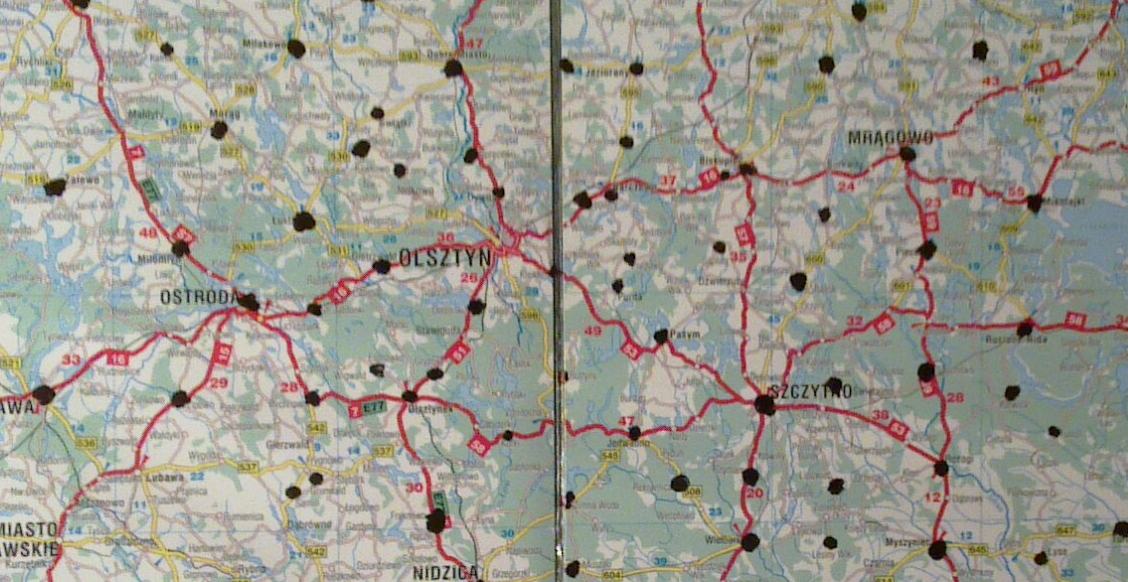
\includegraphics[scale=0.25]{mapa_punkty_zwrotne.eps}
\end{center}
Jeżeli chcesz wykonać przelot warunkowy 50 km to pamiętaj, że 50 km dotyczy
boku trasy. Twoja trasa musi zawierać bok długości co najmniej 50 km.
Jeżeli natomiast atakujesz przelot 300 km to ograniczenia są takie, że
trasa tego przelotu musi być albo trójkątem, albo docelowo-powrotna

Dobrze jest w tym momencie zasięgnąć opinii Szefa Wyszkolenia i innych
doświadczonych szybowników.

\textit{Przykład.} Trasa docel-powrót 119 km Olsztyn-Lipowiec-Olsztyn.
Zawiera bok o długości $> 50$ km, zatem nadaje się do srebrnej odznaki.
Trasę nanosimy na mapę, zaznaczamy kierunki. W połączeniu z kółkami
dolotowymi wygląda to mniej więcej tak:
\begin{center}
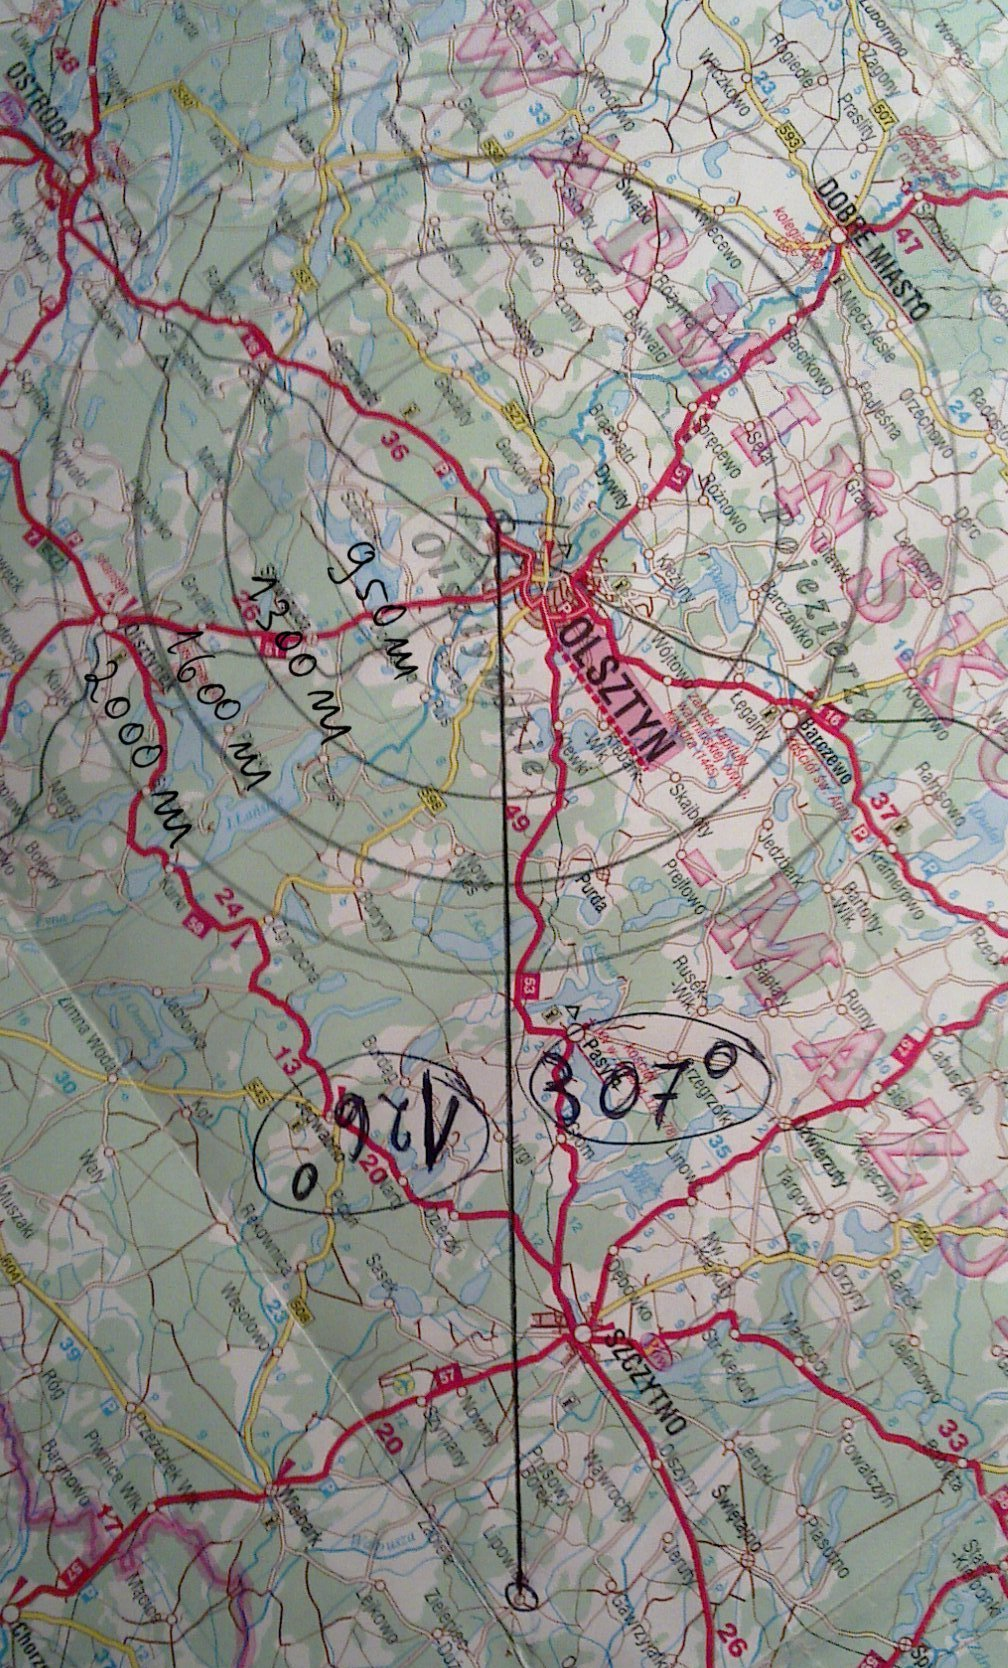
\includegraphics[scale=0.30]{mapa_przelotowa.eps}
\end{center}

\noindent
Przykład mapy gotowej do przelotu. Mapę trzymamy kursem do góry, tu
wybrany został kierunek z Lipowca do Olsztyna (a więc powrotny).


\newpage

\section{Taktyka przelotowa}
Kilka porad.
\begin{itemize}
\item Gdy cumulusy są duże, noszenia występują najczęściej po stronie
    nawietrznej/nasłonecznionej. To znaczy po
    południowo-zachodniej stronie chmury.

\item Gdy cumulusy są małe, płaskie, szybko znikają -- zazwyczaj oznacza
    to, że inwersja występuje w pobliżu poziomu kondensacji. Wtedy zupełnie
    nie opłaca się wznosić się aż do podstawy gdyż noszenie stanie się
    dużo słabsze.

\item Nawet jeżeli widzisz, że chmury są wybudowane i warstwa inwersji jest
    dużo powyżej podstaw, to i tak często nie opłaca się wykorzystywać komina
    do końca. Zazwyczaj najsilniejsze noszenie znajduje się sporo poniżej
    podstawy chmury. Wizualizuje to przykładowe wyjście ze znakomitej
    prognozy TOPTHERM:
    \begin{center}
    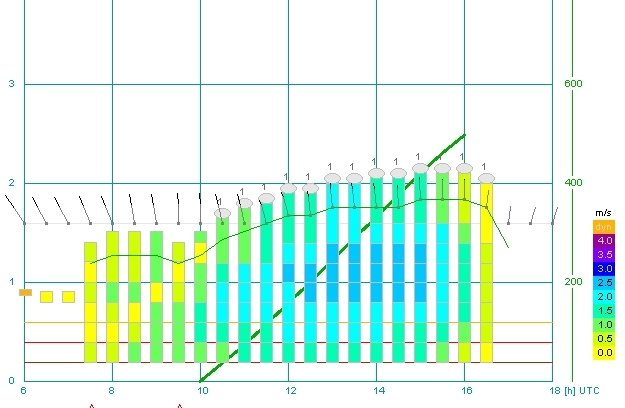
\includegraphics[scale=0.5]{toptherm_przyklad.eps}
    \end{center}
    \noindent
    Widać, że (w tym konkretnym przypadku!) najkorzystniejsze warunki
    można spotkać na wysokościach 700-1500m, przy podstawach
    nieznacznie przekraczających 2000m

\item Krążąc pod wiatr możesz tracić wysokość dolotową. Jeżeli komin jest
    słaby, to próby naboru wysokości mogą nie wystarczyć na pokonanie
    odległości o jaką wiatr przesunął szybowiec. 

\item Niejako wnioskiem z powyższej obserwacji jest pewien sposób nabierania
    wysokości w pobliżu punktu zwrotnego. Jeżeli dolatujesz do punktu
    pod wiatr, napotykasz noszenie przed zaliczeniem punktu zwrotnego,
    to korzystniej jest zakrążyć w tym miejscu po zaliczeniu punktu.
    Wówczas wiatr będzie przybiżał cię do celu.

\item Stosuj teorię McCready'ego. To znaczy, wychodząc z komina ustaw krążek
    na spodziewaną wartość noszenia w następnym kominie. Wyjątkiem jest
    sytuacja, gdy następna chmura jest daleko. Wówczas należy ustawić
    krążek na 0 (czyli maksymalny zasięg względem powietrza).
    Pamiętaj też o wpływie wiatru!
    Ogólna zasada mówi, że lecąc pod wiatr dodajemy połowę prędkości
    wiatru do prędkości wskazywanej przez krążek przelotowy.

\item Przed odejściem na trasę dokładnie sprawdź warunki. Nie nabieraj
    wysokości podstawy w jednym kominie. Wykręć kilkaset metrów w pierwszym,
    przeskocz do innego. Zapamiętaj miejsca w których
    znajdujesz najlepsze noszenia. Krążenie w jednym kominie może dać
    mylne przekonanie o występowaniu silnych warunków.

\item Krążenie kosztuje! Dobrze się zastanów zanim zakrążysz. Każde
    okrążenie to około 15-20 sekund czasu. Na krótkich trasach jedno
    kółko potrafi zmniejszyć prędkość przelotową o ponad $1\frac{km}{h}$.
\end{itemize}
\newpage

\section{Lądowanie w terenie przygodnym}
\subsection{Wybór pól}
Jeżeli znajdziesz się nisko (500 metrów AGL lub niżej) musisz wybrać pola
do lądowania (tak, tak: pola a nie jedno pole).
Dalsze czynności powinieneś/powinnaś
wykonywać pozostając w stożku dolotowym do pól. Decyzja o przerwaniu
poszukiwania noszeń należy do pilota, jednak uczeń-pilot zobowiązany jest
podjąć ją na co najmniej 300 metrach AGL. Ponieważ lądowanie w polu 
jest czynnością stresującą (w szczególności pierwsze lądowanie)
pilot powinien postępować według dobrze zrozumianego
sposobu. Czyli, od momentu znalezienia się na 500-metrach:
\begin{enumerate}
\item Określasz siłę i kierunek wiatru. \\
    Na ogół pilot szybowcowy w tym momencie już posiada
    wystarczające informacje na ten temat odczytując je z lusterka i/lub
    odczuwając wpływ wiatru podczas krążenia. Niemniej dobrymi wskaźnikami są:
    powierzchnia jeziora, wszelkiego rodzaju dymy. Jeśli siła wiatru jest
    znikoma (poniżej $3\frac{m}{s} \approx 10\frac{km}{h}$) to wpływ
    wiatru można pominąć -- lądowanie w polu wymaga koncentracji uwagi
    na innych, ważniejszych sprawach.

\item Wybierasz pola zwracając uwagę głównie na ich rozmiary i przeszkody na
    podejściu, mniej na rodzaj uprawy.\\
    Z obserwacji autora: lądowanie
    na polu z niekorzystną uprawą nie jest tak niebezpieczne jak lądowanie
    na polu za krótkim, z wysokim podejściem czy poprzecinanym drutami.
    Jeżeli wiatr jest istotnym czynnikiem, a teren jest płaski
    to rozważasz tylko jeden kierunek podejścia: pod wiatr. Natomiast
    w terenie górzystym należy lądować wyłącznie pod stok, niezależnie
    od kierunku wiatru.

\item \begin{bf}Bardzo starannie szukasz drutów\end{bf} na wybranych
    polach.\\
    Druty na podejściu absolutnie dyskwalifikują pole jako lądowisko.
    Fakty są takie, że w okolicach Olsztyna prawie każde pole jest
    przecięte drutami.

\item Jeżeli pól jest pod dostatkiem to możesz wybrać pole o najlepszej
    powierzchni. \\
    Najlepsze powierzchnie to:
    \begin{enumerate}
        \item Pola zaorane \\
            Poznać je można po czarno-brązowym kolorze
        \item Ścierniska \\
            Są dobre o ile tylko nie występuje na nich słoma w postaci bali.
            Kolor brązowy, prześwitują żółte pozostałości po zbożu.
        \item Niska uprawa \\
            Czyli między innymi: wczesna kukurydza, kapusta, buraki, świeżo
            posiane zboże. Wygląd: zielone grządki między którymi
            widać ciemniejszą ziemię.
    \end{enumerate}
\end{enumerate}

\subsection{Podejście do lądowania w polu}
Jeżeli poszukiwania noszeń zawiodły powinieneś/powinnaś:
\begin{enumerate}
\item Wejść do pozycji ,,z wiatrem'' \\
    względem planowanego punktu przyziemienia.
    Dobra wysokość dla tej fazy lotu to
    200-300m AGL. Pojawia się istotny szczegół: \begin{bf}pozycja z
    wiatrem powinna wypaść około 200-500m obok osi lądowania.\end{bf}
    Jest to ważne, ponieważ przelatując zbyt blisko nad polem nie
    zauważysz nierówności terenu. Przelatując nad samym polem w ogóle
    go nie obejrzysz. 

\item Ponownie obejrzeć pole\\
    i ewentualnie skorzystać z innych wybranych pól. Różnica jest taka,
    że tym razem jesteś dużo niżej i być może dopiero
    teraz widać nierówności terenu lub druty uniemożliwiające bezpieczne
    lądowanie.

\item Wyjść na prostą\\
    w dobrej odległości. Dobrej czyli też nie za małej. Zawracanie na
    krawędzi krótkiego pola jest złym pomysłem, możesz się nie zmieścić.

\item Wykonać esowanie, jeżeli znajdziesz się za wysoko.\\
    Pamiętaj o zasadzie esowania: zakręty wykonujemy w stronę
    lądowiska.

\item Wylądować.\\
    Jeżeli pole jest krótkie powinnaś/powinieneś zminimalizować energię
    szybowca -- 
    przelecieć kilka metrów nad ostatnią przeszkodą, na możliwie małej
    prędkości (dostosowanej do typu szybowca i turbulencji).

\end{enumerate}

\subsection{Postępowanie po lądowaniu}
Zadzwoń do kolegów i zrelaksuj się, spędzisz w tym miejscu ładnych
kilka godzin~:).
A tak na poważnie, zacznij od przeglądu szybowca, skupiając swoją
uwagę na (ewentualnych) pęknięciach i zarysowaniach na kadłubie.
Pamiętaj, że inny pilot może być zmuszonym do lądowania na twoim polu, zatem
poproś widzów o pomoc w transporcie szybowca na skraj pola. Przydatna
może okazać się linka którą radziłem zabrać ze sobą. Skorzystaj z
telefonu informując Aeroklub o fakcie lądowania, stanie szybowca i planach
powrotu.

\subsection{Postępowanie w przypadku uszkodzenia szybowca}
Jeżeli są ofiary wypadku to w pierwszej kolejności wykonaj telefon na numer
alarmowy (112 lub 999). Zabezpiecz teren wokół szybowca (tak, aby dało się
zebrać konieczne dowody). Poinformuj Aeroklub i Państwową Komisię Badania
Wypadków Lotniczych. Wykonaj serię zdjęć jeżeli masz aparat fotograficzny.

\newpage
\section{Dodatki}
\subsection{Schemat montażu/demontażu Pirata}

\noindent
Tok pracy przy montażu:
\begin{enumerate}
\item Otworzyć limuzynę i wyjąć sworznie główne. Zdjąć pokrywę
   grzbietową. Wyjąć sworznie nośne.
\item Oczyścić i nasmarować wazeliną techniczną powierzchnie robocze okuć,
   sworzni, gniazd oraz złącz napędów.
\item Przytrzymać kadłub i nałożyć odpowiednio środkową część skrzydła.
   Założyć sworznie główne i zabezpieczyć rękojeści zasuwkami. Połączyć
   napęd lotek i założyć agrafkę. Połączyć i zabezpieczyć napęd hamulców
   aerodynamicznych.
\item Zaśrubować klucz montażowy z jednym ze sworzni nośnych. Zestawić
   odpowiednio zewnętrzną część skrzydła, aż do pokrycia się okuć,
   następnie założyć sworzeń nośny. Ustawić otworek sworznia w
   płaszczyźnie lotu i założyć agrafkę zabezpieczającą (od przodu do tyłu).
   Zwolnić klucz montażowy. Połączyć i zabezpieczyć napęd lotki
   (przez wziernik w dolnej powierzchni skrzydła). \\
\begin{tabular}{|l|}
\hline
Uwaga: \\
  SWORZEŃ NOŚNY MOŻNA ZAKŁADAĆ TYLKO ZA POMOCĄ \\
  KLUCZA, PRZEZ WCISKANIE Z JEDNOCZESNYM OBROTEM \\
  WAHADŁOWYM. WBIJANIE MŁOTKIEM JEST NIEDOZWOLONE!\\
\hline
\end{tabular}

   Podobnie założyć drugą zewnętrzną część skrzydła.
\item Ustawić w pobliżu neutrum klapkę wyważającą oraz jej suwak w
   kabinie. Zaśrubować klucz montażowy ze śrubą mocującą usterzenie
   wysokości i nałożyć usterzenie na okucie [1] i gniazdo [3]. Napęd klapki
   wyważającej łączy się samoczynnie. Wkręcić śrubę mocującą [4] i
   dociągnąć ją siłą jednej ręki poruszając lekko usterzeniem wysokości.
   Śrubę dociągnąć aż do zlikwidowania luzu. Po dociągnięciu, ramię
   klucza powinno być ustawione w płaszczyźnie symetrii szybowca. lub
   prostopadle do niej.
\item Zdjąć klucz i zamknąć wieczko. Do wkręcenia wkręta zabezpieczającego
   użyć śrubokręta.
\item Połączyć i zabezpieczyć napęd steru wysokości.
\item Sprawdzić wszystkie połączenia oraz poruszyć kilkakrotnie napędami
   sterów, hamulców i klapki wyważającej. Zamknąć wzierniki i założyć
   pokrywę grzbietową.
\end{enumerate}

\newpage
\noindent
Tok pracy przy demontażu:
\begin{enumerate}
    \item Rozłączyć napędy:
    \begin{itemize}
        \item centralne (złącza napędów lotek i hamulców są dostępne po
             zdjęciu pokrywy grzbietowej),
        \item zewnętrzne lotkowe (przez dolne wzierniki skrzydłowe),
        \item steru wysokości (złącze przy sterze wysokości).
    \end{itemize}
    \item Otworzyć wieczko na usterzeniu wysokości, założyć klucz montażowy,
         wykręcić śrubę i zdjąć usterzenie.
    \item Odbezpieczyć sworzeń nośny dowolnego skrzydła (zdjąć agrafkę) i
         założyć klucz montażowy. Przytrzymać (odciążyć) demontowaną część
         skrzydła oraz końce obu skrzydeł i wyciągnąć sworzeń nośny. Zdjąć
         zewnętrzną część skrzydła. Sworzeń założyć z powrotem, do okuć części
         środkowej i zabezpieczyć agrafką. Podobnie zdemontować drugą
         zewnętrzną część skrzydła.
    \item Odbezpieczyć i wyciągnąć sworznie główne. Zdjąć środkową część
         skrzydła. Sworznie założyć z powrotem do okuć kadłuba i zabezpieczyć
         zasuwkami.
\end{enumerate}

\newpage
\subsection{Montaż usterzenia wysokości Pirata}

\begin{center}
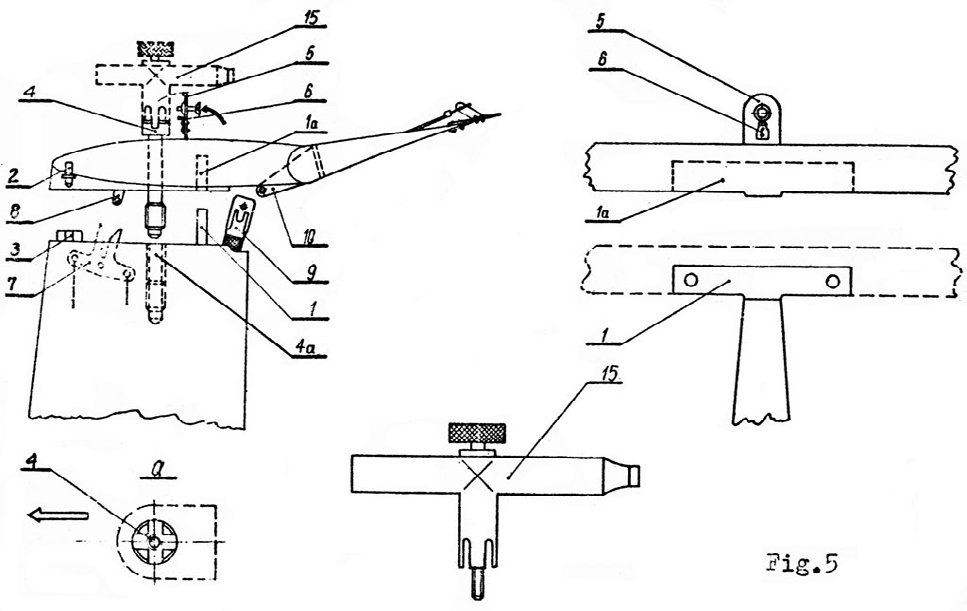
\includegraphics[scale=0.38]{montaz_usterzenia_wysokosci_pirat.eps}
\end{center}

\begin{packed_enum}
\item[1] -- okucie duralowe ,,T''
\item[1a] -- gniazdo okucia ,,T''
\item[2] -- czop przedni
\item[3] -- gniazdo czopa
\item[4] -- śruba mocująca
\item[4a] -- gniazdo śruby
\item[5] -- wieczko zawiasowe z wkrętem
\item[6] -- palec zabezpieczający
\item[7] -- widelec napędu klapki wyważającej
\item[8] -- dźwigienka napędu klapki wyważającej
\item[9] -- popychacz napędu steru wysokości ze złączem
\item[10] -- dźwigienka steru wysokości
\item[15] -- klucz montażowy ze śrubą i śrubokrętem
\item[a)] -- właściwe ustawienie śruby mocującej przed zamknięciem
wieczka (wykroje dla klucz ustawione w płaszczyźnie symetrii
szybowca).
\end{packed_enum}

\newpage
\subsection{Montaż skrzydła Pirata}

\begin{center}
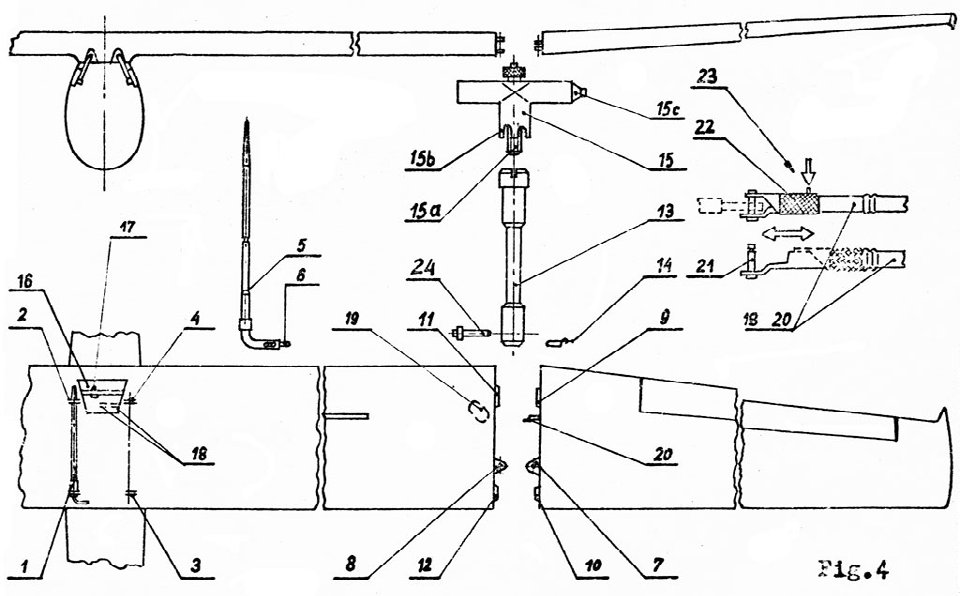
\includegraphics[scale=0.36]{montaz_skrzydel_pirat.eps}
\end{center}

\begin{packed_enum}
\item[1, 2] -- prawa para okuć głównych
\item[3, 4] -- lewa para okuć głównych
\item[5] -- sworznie główne
\item[6] -- zasuwki zabezpieczające
\item[7] -- okucie nośne zewnętrznej części skrzydła
\item[8] -- okucie nośne środkowej części skrzydła
\item[9, 10] -- okucia zderzakowe zewnętrznej części skrzydła
\item[11, 12] -- okucia zderzakowe środkowej części skrzydła
\item[13] -- sworzeń nośny
\item[14] -- agrafka
\item[15] -- klucz montażowy „T”
\item[15a] -- śruba z pokrętłem
\item[15b] -- zęby robocze
\item[15c] -- śrubokręt
\item[16] -- pokrywa grzbietowa
\item[17] -- popychacz napędu lotek ze złączem i agrafką
\item[18] -- złącza napędów hamulców
\item[19] -- wziernik na dolnej powierzchni skrzydła
\item[20] -- popychacz ze złączem napędu lotki
\item[21] -- czop złącza
\item[22] -- tuleja z ramieniem widełkowym
\item[23] -- zatrzask
\item[24] -- przetyczka
\end{packed_enum}

\newpage
\subsection{Schemat montażu/demontażu skrzydeł Juniora}

\begin{center}
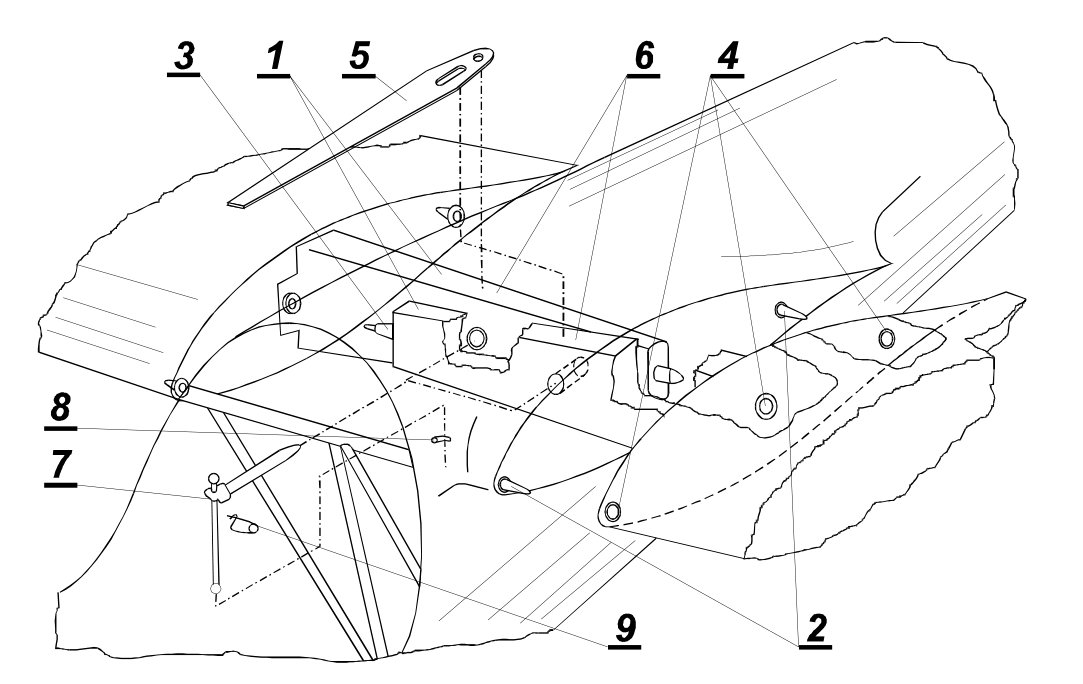
\includegraphics[scale=0.36]{montaz_skrzydel_junior.eps}
\end{center}

\begin{packed_enum}
\item[1] -- trzony dźwigarów skrzydeł
\item[2] -- czopy kadłuba
\item[3] -- czopy dźwigarów
\item[4] -- gniazda czopów
\item[5] -- dźwignia montażowa
\item[6] -- stopki oporowe dźwigarów
\item[7] -- sworzeń
\item[8] -- otwór zabezpieczający
\item[9] -- agrafka
\end{packed_enum}

\noindent
Schemat montażu:
\begin{enumerate}
\item Przestawić suwak hamulców aerodynamicznych w kabinie do przodu
   drążek ustawić w płaszczyźnie symetrii.
\item Hamulce aerodynamiczne schować, lotki ustawić w neutrum.
\item Prawe a następnie lewe skrzydło zestawić z kadłubem. Podczas wsuwania
   trzonów dźwigarowych [1] wystające czopy dźwigarów i kratownicy
   kadłuba [3] muszą wejść w odpowiednie gniazda [4] na żebrach przy-
   kadłubowych skrzydeł. Również muszą się połączyć złącza napędów lotek
   i hamulców aerodynamicznych.
\item Dźwignię montażową [5] założyć na stopki oporowe [6] dźwigarów i
   dociągnąć ostatecznie obydwa skrzydła do kadłuba.
\item Połączyć dźwigary sworzniem [7], poprzeczkę sworznia wprowadzić do
   otworu [8] i zabezpieczyć agrafką [9].
\end{enumerate}

\noindent
Demontaż skrzydeł: w kolejności odwrotnej do montażu wyjąć
sworzeń [7] i zdjąć skrzydła.

\newpage
\subsection{Schemat montażu/demontażu usterzenia wysokości Juniora}

\begin{center}
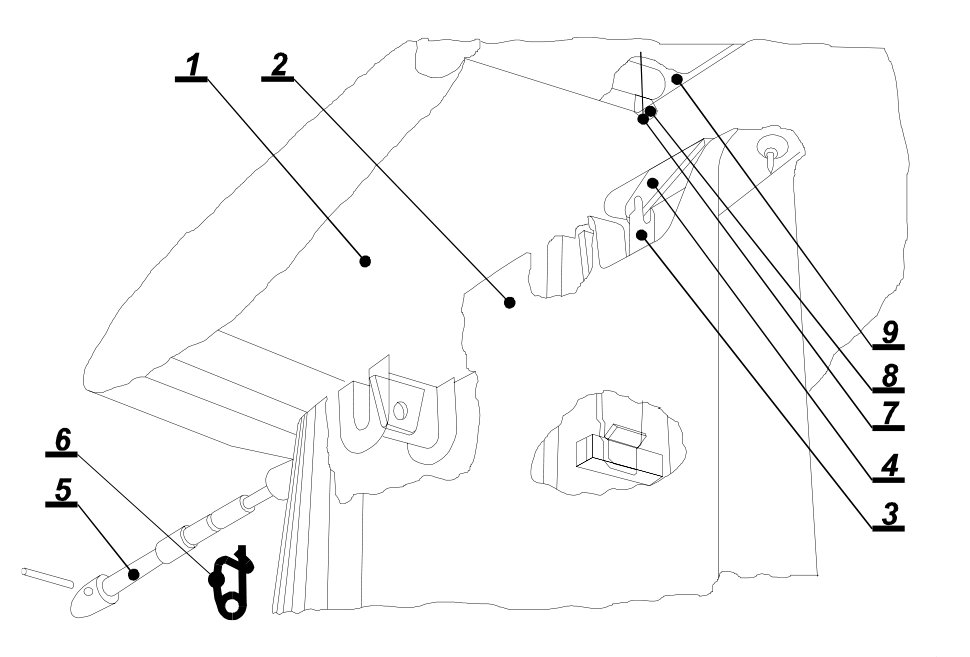
\includegraphics[scale=0.38]{montaz_usterzenia_wysokosci_junior.eps}
\end{center}

\begin{packed_enum}
\item[1] -- usterzenie wysokości,
\item[2] -- statecznik kierunku,
\item[3] -- końcówka szybkorozłączna,
\item[4] -- dźwigienka steru wysokości,
\item[5] -- sworzeń,
\item[6] -- agrafka,
\item[7] -- śruba mocująca ster wysokości
\end{packed_enum}

\noindent
Schemat montażu:
\begin{enumerate}
\item Uchwyt urządzenia wyważającego w kabinie przestawić do przodu.
\item Nałożyć usterzenie [1] na statecznik kierunku.
\item Połączyć złącze popychacza [3] z dźwignią steru wysokości [4].
\item Połączyć okucia przez wprowadzenie sworznia [5] w otwór w krawędzi
    natarcia statecznika pionowego i zapiąć agrafkę [6].
\end{enumerate}

\noindent
Demontaż usterzenia wysokości: W kolejności odwrotnej wyjąć sworzeń [5],
rozłączyć złącze napędu [3] i zdjąć usterzenie wysokości.

\end{document} 
